% !Mode:: "TeX:UTF-8"
% !TEX program  = xelatex
\documentclass[a4paper]{article}
\usepackage{amsmath}
\usepackage{amssymb}
\usepackage{ctex}
%\usepackage{braket}
%\usepackage[european]{circuitikz}
\usepackage{multirow}
\usepackage{float}
\usepackage{graphicx}
\usepackage{geometry}
\geometry{left=2.5cm,right=2.5cm,bottom=2.5cm,top=2.5cm}
\title{近代物理实验报告11.4:矢量网络分析仪测量微波材料的节电常量和磁导率}
\author{林杨\quad 211840092\quad 物理学院}
\date{2024年11月14日}
\begin{document}
\maketitle
\bibliographystyle{unsrt}
%--------main-body------------

\section{引言}
微波装置和器件中应用了许多类型的介质材料。电介质的应用极为广泛,例如,同轴线中的绝缘片、条形线中的介质条、加载波导中的介质块、介质天线中的介质杆、天线的介质外罩以及各种器件的支持装置和密封窗孔等等。近年来,微波隐身技术得到了很大的发展,其中涂覆型隐身技术是将吸波材料直接以一定的厚度涂覆在外壳以降低对微波的反射,减少雷达探测面积,提高隐身能力。现已应用到导弹、飞机、舰船、装甲车辆、重要军事设施等许多武器装备上。介质的特性与微波装置和器件的技术性能,材料的吸波性能有着密切的关系。因此,在微波频率测量介质的特性参量是有实际的重要意义的。\\
矢量网络分析仪是一种性能优越的测量仪器,能够对网络参数进行全面测量。本实验利用矢量网络分析仪扫频测量装有微波材料样品的二端口网络的散射系数(s参数),采用传输/反射法推出待测样品的介电常数和磁导率随s参数变化的公式,从而计算得到样品材料的介质特性随频率的变化趋势。

\section{实验目的}
\begin{enumerate}
\item 了解矢量网络分析仪的操作和使用。
\item 掌握矢量网络分析仪测量s参数的原理和方法。
\item 掌握传输/反射法由s参数计算介电常数和磁导率的过程和方法。
\end{enumerate}

\section{实验仪器}
高性能微波一体化矢量网络分析仪、样品。

\section{实验原理}
矢量网络分析仪能够对网络参数进行全面测量,它既可测量网络的幅频特性,又可测量网络的相频特性和群延迟特性。可广泛应用于天线和雷达散射截面RCS测量,发射/接收(T/R)模块测量,介质材料特性测量,微波脉冲特性测量,光电特性测量和低温电子测量等领域,是相控阵雷达、精密制导、电子对抗、隐身和反隐身技术、微波通信和卫星等电子系统的科研、生产过程中必不可少的测试设备。\\
矢量网络分析仪的工作原理:矢量网络分析仪的信号源产生测试信号输入到被测件,当测试信号通过被测件时,一部分信号被反射,另一部分信号则被传输,那么反射和传输信号就携带了被测件的特征信息,矢量网络分析仪通过测量反射和传输信号得到被测件的特征参量。\\
矢量网络分析仪AV3629用于测量器件和网络的反射和传输特性。整机主要包括45MHz-40GHz合成信号源、53MHz-24GHz本振源、s参数测试装置模块、幅相接收模块、数字信号处理与嵌入式计算机模块和液晶显示模块。合成信号源产生45MHz-40GHz的测试激励信号,此信号通过整机锁相电路与本振源同步扫描。s参数测试装置模块用于分离被测件的入射信号、反射信号和传输信号。当源在端口1时,产生入射信号R1、反射信号A和传输信号B;当源在端口2时,产生入射信号R2、反射信号B和传输信号A。幅相接收模块将射频信号转换成固定频率的中频信号,由于采用系统锁相技术,本振源和信号源锁相在同一个参考时基上,保证在频率变换过程中,被测件的幅度和相位信息不丢失。在数字信号处理与嵌入式计算机模块中,将模拟中频变成数字信号,通过计算得到被测件的幅相信息,这些信息做各种格式变换处理后,将结果送给显示模块,液晶显示模块将被测件的幅相信息以用户需要的格式显示出来。\\
\begin{figure}[!h]
\centering
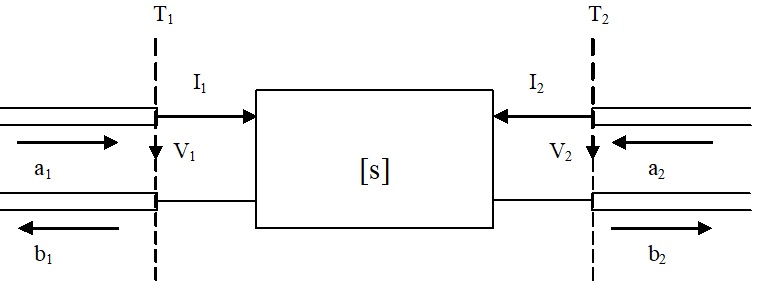
\includegraphics[width=12cm]{fig/2port.jpg}\\
\caption{二端口网络}\label{2port}
\end{figure}
实验中待测样品材料通过同轴波导转换器接在矢量网络分析仪端口1和端口2之间。根据微波网络理论,本实验实际上是测量一个二端口网络的s参数,如图(\ref{2port})所示,$a_1$、$a_2$和$b_1$、$b_2$分别是端口1和端口2的内向波和外向波;$T_1$和$T_2$分别为端口1和端口2的参考面;$V_1$、$I_1$和$V_2$、$I_2$分别端口1和端口2的归一化电压和电流。\\
外向波与内向波和s参数之间的关系可表示为:
\begin{equation}
\begin{bmatrix}
b_1 \\
b_2
\end{bmatrix}
= 
\begin{bmatrix}
s_{11} & s_{12}\\
s_{21} & s_{22}
\end{bmatrix}
\begin{bmatrix}
a_1\\
a_2
\end{bmatrix}
\end{equation}
其中,
\begin{equation}
s_{11} = \left.\frac{b_1}{a_1}\right|_{a_2=0}, 
s_{12} = \left.\frac{b_1}{a_2}\right|_{a_1=0}, 
s_{21} = \left.\frac{b_2}{a_1}\right|_{a_2=0}, 
s_{22} = \left.\frac{b_2}{a_2}\right|_{a_2=0}
\end{equation}
$s_{11}$表示端口1的反射系数,$s_{12}$表示端口2到端口1的传输系数,$s_{21}$表示端口1到端口2的传输系数,$s_{22}$表示端口2的反射系数。\\
本实验两端口网络具有对称性,因此有$s_{11}=s_{22}$, $s_{12}=s_{21}$。\\
根据传输/反射法,在矩形波导传输线中包含样品时,微波在空气—介质界面要发生反射和透射,s参数与反射系数和传输系数有关,可以得到:
\begin{eqnarray}
s_{11} &=& s_{22} = \cfrac{\Gamma_c(1-T_l^2)}{1-\Gamma^2T^2_l}\label{eq1}\\
s_{12} &=& s_{21} = \cfrac{T_l(1-\Gamma_c^2)}{1-\Gamma_c^2T_l^2}\label{eq2}
\end{eqnarray}
其中,$T_l$表示待测样品的传输系数,$\Gamma_c$表示待测样品的反射系数。
由式(\ref{eq1})、(\ref{eq2}),令
\begin{equation}
K = \cfrac{s_{11}^2-s_{12}^2+1}{2s_{11}}
\end{equation}
可以得到
\begin{eqnarray}
\cfrac{s_{11}^2-s_{12}^2+1}{2s_{11}} &=& \cfrac{1+\Gamma_c^2}{2\Gamma_c}\\
\Gamma_c &=& K\pm\sqrt{K^2-1}
\end{eqnarray}
其中$\pm$号的选择依据是满足$|\Gamma_c|<1$
\begin{equation}
T_l = \cfrac{s_{21}}{1-\Gamma_c\cdot s_{11}}
\end{equation}

同时考虑到材料样品的传输系数$T_l$可以通过传播常数$\gamma$与材料的电磁参数$\varepsilon_r$,$\mu_r$联系起来,即
\begin{eqnarray}
T_l &=& e^{-\gamma l}\\
\gamma &=& j\cfrac{2\pi}{\lambda_0}\sqrt{\mu_r\varepsilon_r-\left(\frac{\lambda_0}{\lambda_c}\right)^2}
\end{eqnarray}
其中,$l$为待测样品厚度,$\gamma$为样品区的传播常数,$c$为光速,$\lambda_0$为空气中的工作波长,$\lambda_0 = \frac{c}{f}$,$\lambda_c$为截止波长。
空气—介质界面的反射系数$\Gamma_c$也可以通过波阻抗与材料的电磁参数$\varepsilon_r$,$\mu_r$联系起来,即
\begin{eqnarray}
\Gamma_c &=& \cfrac{Z_c-Z_0}{Z_c+Z_0}\\
Z_0 &=& \cfrac{c\mu_0}{\sqrt{1-\left(\frac{\lambda_0}{\lambda_c}\right)^2}}\\
Z_c &=& \cfrac{c\mu_r\mu_0}{\sqrt{\mu_r\varepsilon_r-\left(\frac{\lambda_0}{\lambda_c}\right)^2}}
\end{eqnarray}

其中,$Z_c$和$Z_0$分别代表传输线中样品段和空气段的波阻抗,即有
\begin{equation}
\Gamma_c = \left[\sqrt{1-\left(\frac{\lambda_0}{\lambda_c}\right)^2} - \cfrac{1}{\mu_r}\sqrt{\mu_r\varepsilon_r-\left(\frac{\lambda_0}{\lambda_c}\right)^2}\right]/\left[\sqrt{1-\left(\frac{\lambda_0}{\lambda_c}\right)^2} + \cfrac{1}{\mu_r}\sqrt{\mu_r\varepsilon_r-\left(\frac{\lambda_0}{\lambda_c}\right)^2}\right]
\end{equation}

联合以上各式可以得到
\begin{eqnarray}
\mu_r &=& \cfrac{1}{\Lambda\sqrt{\frac{1}{\lambda_0^2}-\frac{1}{\lambda_c^2}}}\left(\cfrac{1+\Gamma_c}{1-\Gamma_c}\right)\\
\varepsilon_r &=& \cfrac{\left(\frac{1}{\Lambda^2}+\frac{1}{\lambda_c^2}\right)\lambda_0^2}{\mu_r}
\end{eqnarray}
式中,
\begin{equation}
\cfrac{1}{\Lambda^2} = \cfrac{\varepsilon_r\mu_r}{\lambda_0^2} - \cfrac{1}{\lambda_c^2} = -\left[\cfrac{1}{2\pi l}\ln\left(\frac{1}{T_l}\right)\right]^2\label{eq4.17}
\end{equation}
并且有,
\begin{equation}
Re\left(\cfrac{1}{\Lambda}\right) = \cfrac{1}{\lambda_g} > 0\label{eq4.18}
\end{equation}
$\lambda_g$为待测材料中的波导波长。根据式(\ref{eq4.18})来决定式(\ref{eq4.17})开方后的正负号选取。\\
综合上述诸式,只要测得材料样品端面的散射参数$s_{11}$和$s_{21}$,就可以得到界面的反射系数$\Gamma_c$和材料的传输系数$T_l$,继而得到材料的电磁参数$\varepsilon_r$, $\mu_r$。\\
此方法优点,简单且具有较高精度,同时对波导与同轴系统均适用。\\
此方法会产生以下两个问题:
\begin{enumerate}
\item 厚度谐振问题\\
对于低损耗材料,某些频点,即微波材料样品长度正好是半波长的整数倍时,$|s_{11}|\to 0$,$K$值具有极大的不确定性,$\varepsilon_r$产生尖峰,即厚度谐振为不确定值需要去除。
\item 多值问题\\
传播常数与厚度紧密相关,当$l > \lambda$时,传播常数有多个解,在式(\ref{eq4.17})需要对$T_l$取自然对数,设$T_l = Te^{j\theta}$,则有
\begin{equation}
\gamma = -\frac{1}{l}\ln(T_l) = -\frac{1}{l}\left[\ln(T)+j(\theta\pm 2n\pi)\right] \text{ (n=0,1,2...)}
\end{equation}
由于$n$可能取多个不同的值,$\gamma$值存在多个值,因而得到的介电常数可能存在多值。
\end{enumerate}

\section{实验内容}
\begin{enumerate}
\item 打开矢量网络分析仪,预热60分钟。
\item 测量待测材料厚度,波导板的厚度和波导尺寸(多点平均法)。
\item 在矢量网络分析仪上根据波导尺寸设置好扫描频率、点数和扫描时间。
\item 根据波导尺寸,使用矢量网络分析仪的标准件(开路器、断路器、匹配负载、直通)和自带的校准程序对测试系统进行校准:
\begin{enumerate}
\item 打开校准菜单选择校准向导,选择校准类型,点中全双端口SOLT(忽略隔离),然后选择测量机械校准,选择标准件开始进行校准。
\item 将两转换头波导口对接,进行直通校准。
\item 在两转换头波导口分别接上短路板,进行短路校准。
\item 在两转换头波导口分别接上四分之一波长负载进行偏移校准。
\item 在两转换头波导口分别接上精密波导负载进行负载校准。
\item 点“确定”,矢量网络分析仪自动记录校正信息。
\end{enumerate}
\item 在测试程序界面建立四个窗口,分别测试$s_{11}$, $s_{12}$, $s_{21}$, $s_{22}$。
\item 将待测量的微波材料接在两个转换器之间,测量此时的s参数。因为本系统是对称的两端口网络,因此测得的$s_{11}=s_{22}$, $s_{12}=s_{21}$。
\item 把测得的结果存成数据文件。
\item 利用s参数编程计算微波材料的介电常数$\varepsilon_r$和磁导率$\mu_r$随频率的变化。
\end{enumerate}

\section{实验数据}
\begin{itemize}
\item 样品厚度:$l$ = 2.00mm
\item 样品长度:$l_{wg}$ = 7.07mm
\item 所得数据文件:3303.dat
\end{itemize}
实验数据经处理后所得结果如图(\ref{sPara})、(\ref{sssa})、(\ref{final}):
\begin{figure}[!h]
\centering
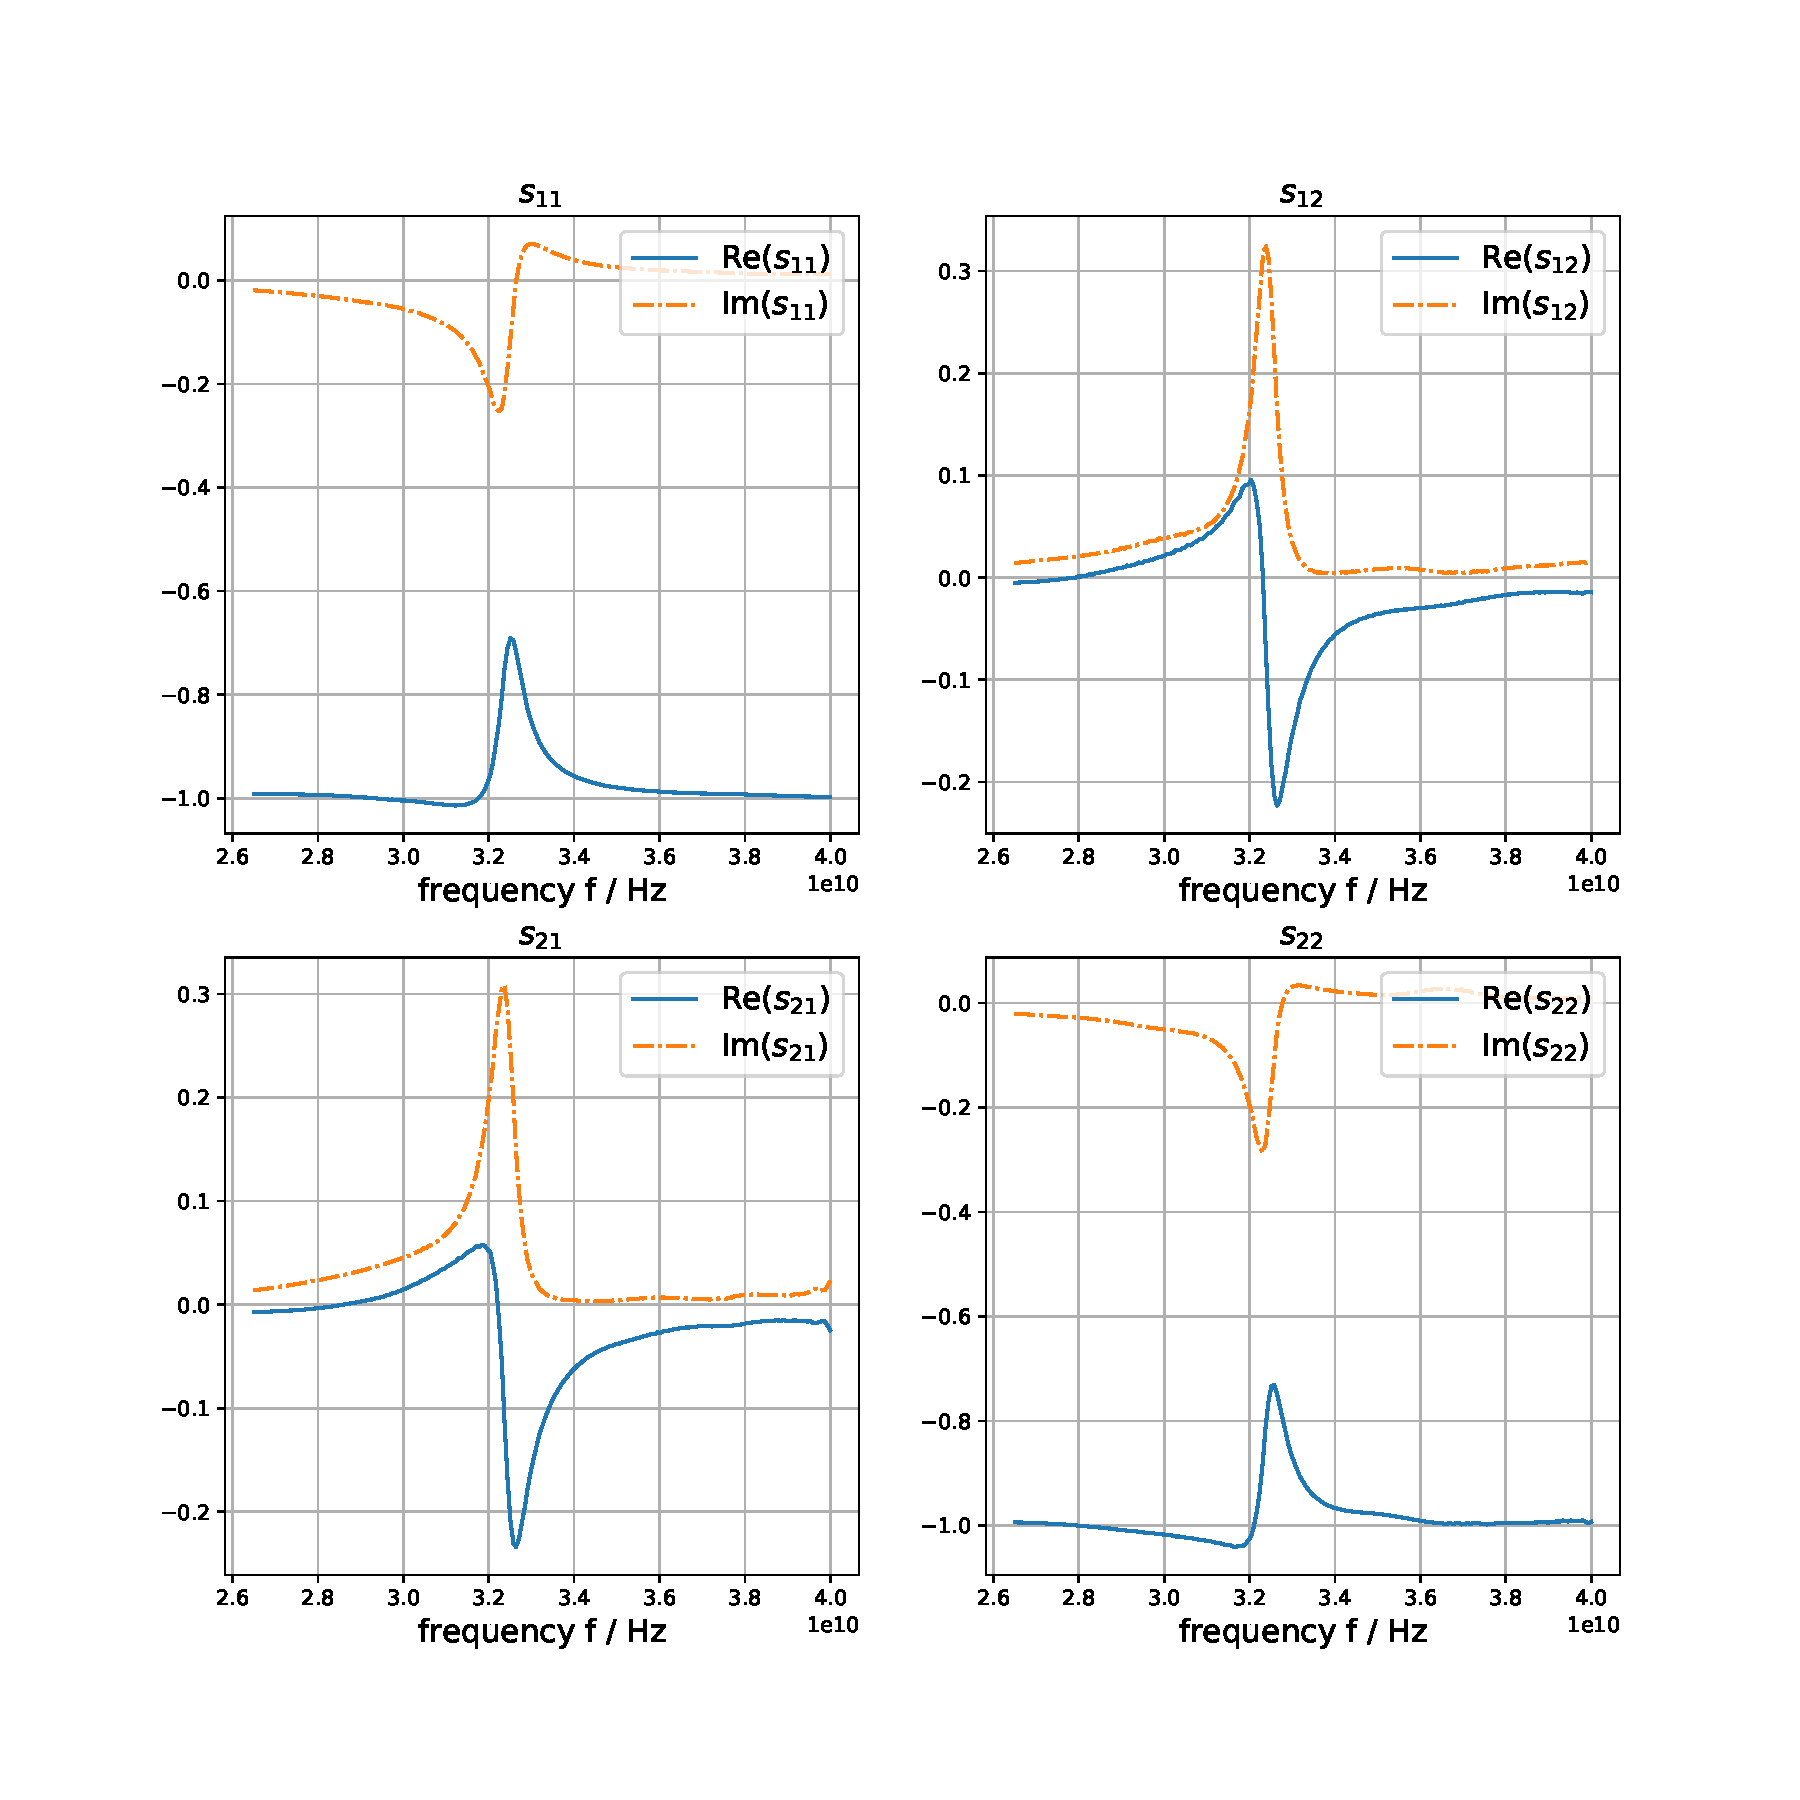
\includegraphics[width=12cm]{fig/sParameter.pdf}\\
\caption{4个s参数}\label{sPara}
\end{figure}
\begin{figure}[!h]
\centering
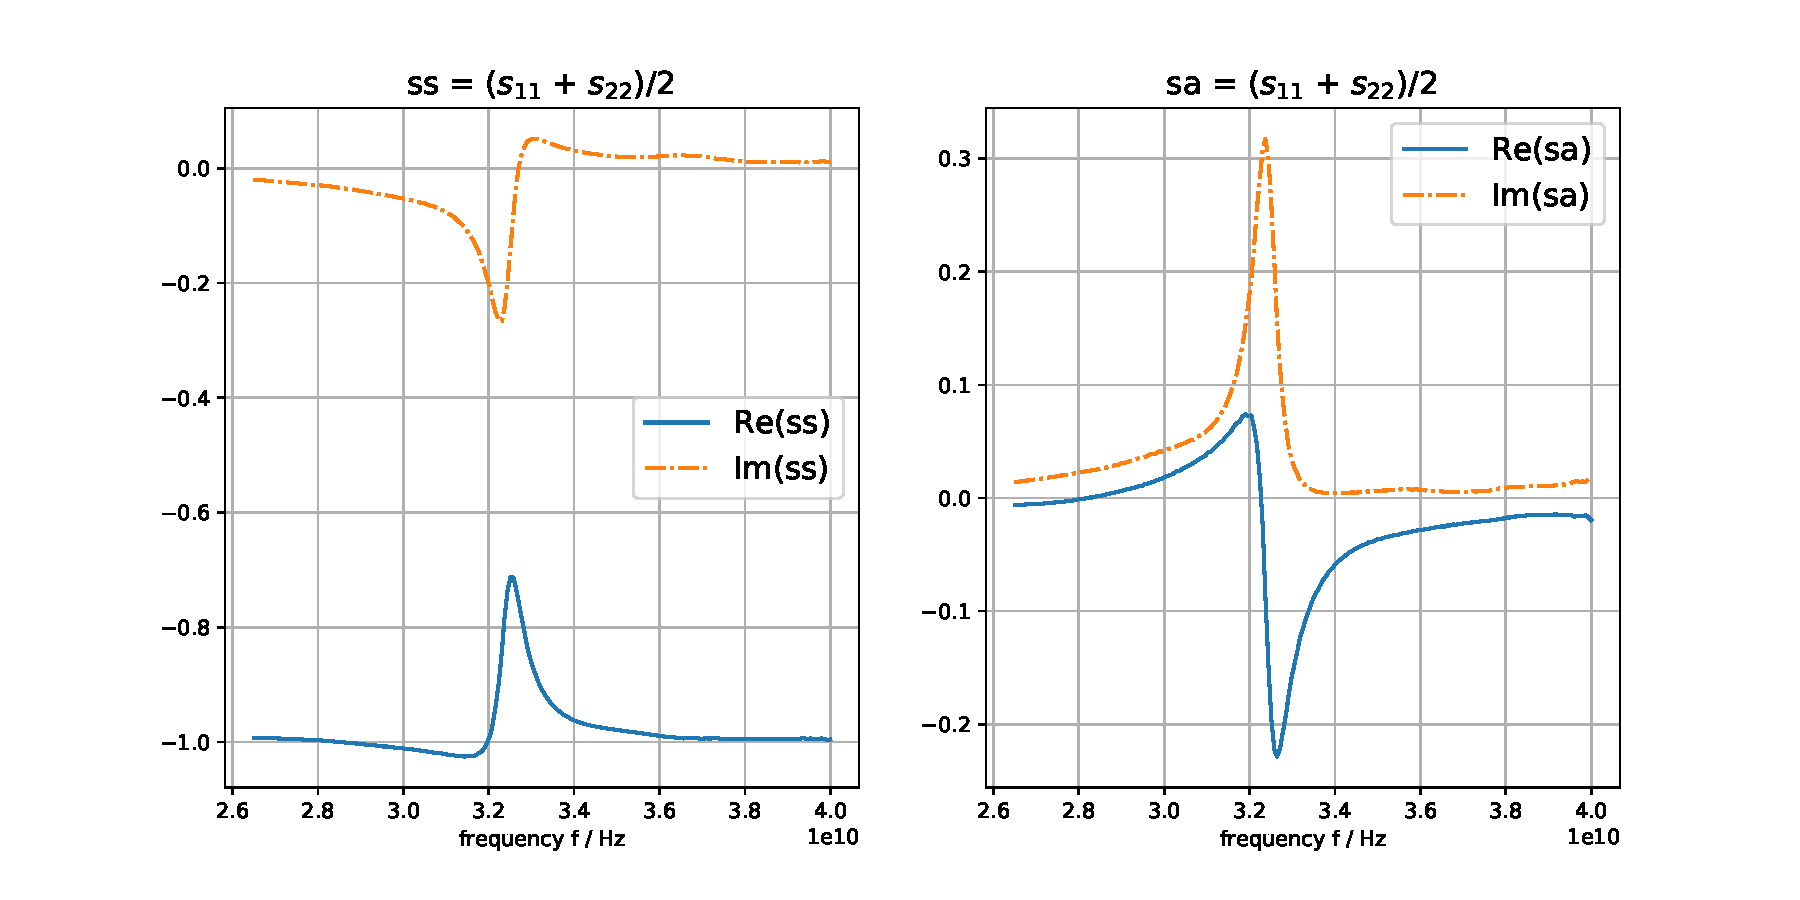
\includegraphics[width=12cm]{fig/sssa.pdf}\\
\caption{取平均数后的$s_{11}$和$s_{12}$}\label{sssa}
\end{figure}
\begin{figure}[!h]
\centering
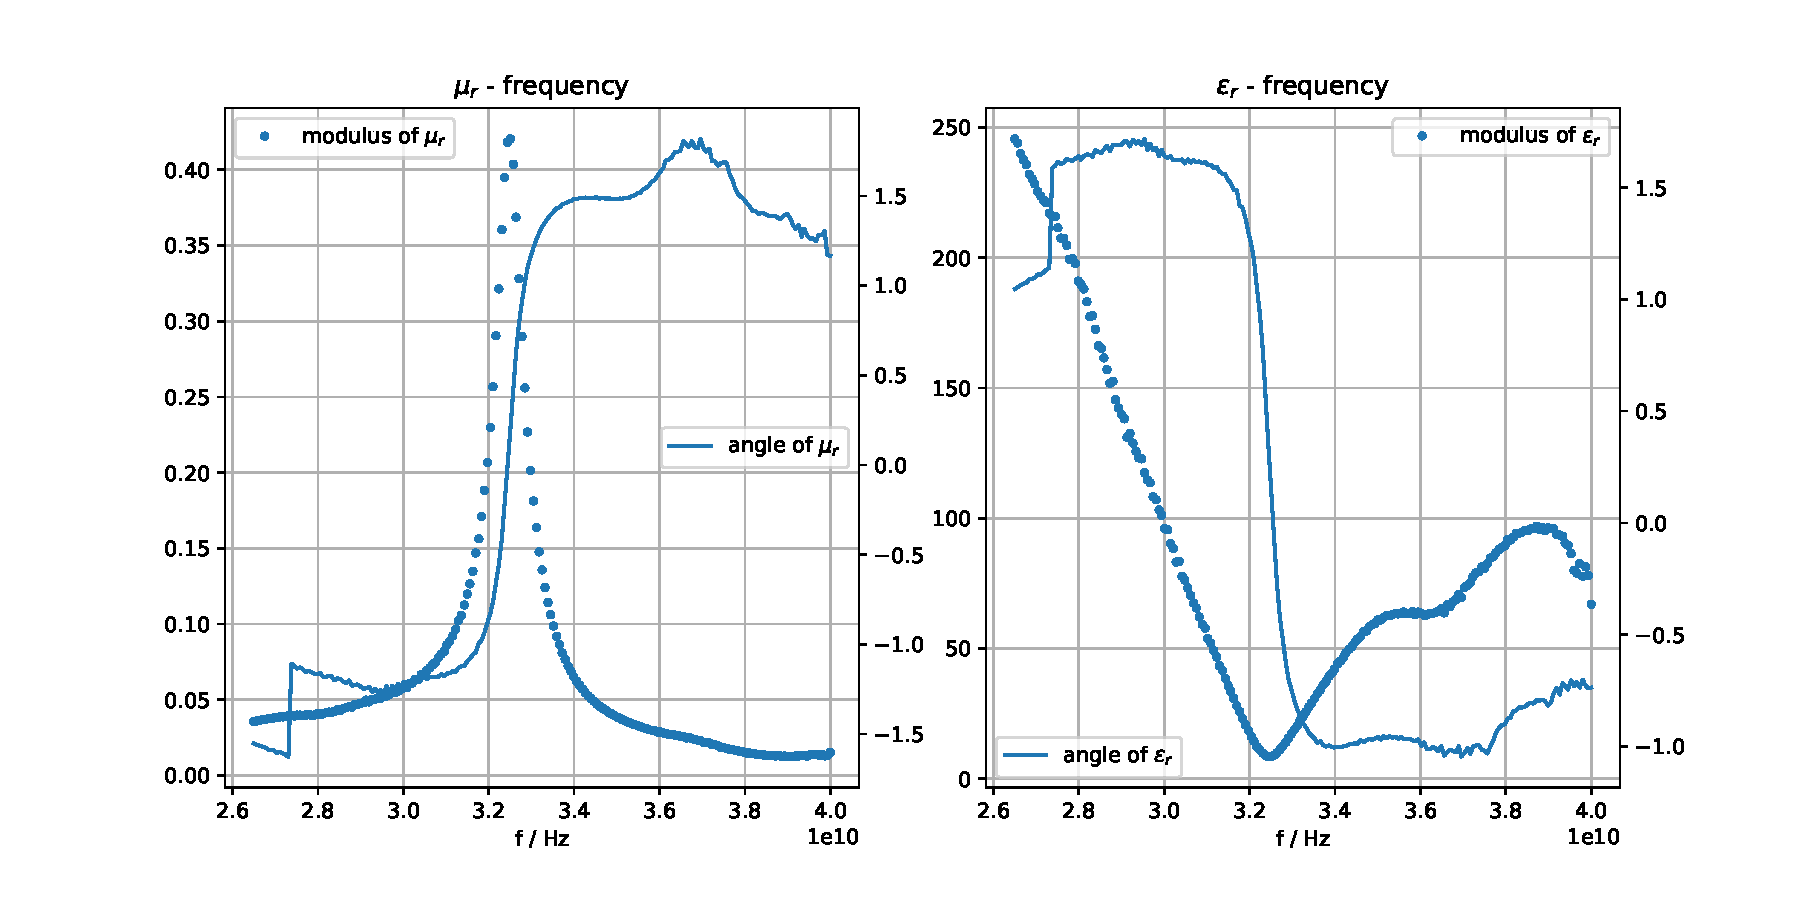
\includegraphics[width=12cm]{fig/final.pdf}\\
\caption{$\mu_r$和$\varepsilon_r$关于信号频率的曲线}\label{final}
\end{figure}

\section{思考题}
\subsection{本实验测得材料的介电常数和磁导率其主要误差来源是什么?}
\subsection{微波材料的隐身特性与材料的涂覆厚度有关,试计算本实验测得的微波材料涂覆在金属平板上,微波垂直入射时反射系数随材料厚度以及频率的变化,考察材料厚度对隐身性能的影响。}

\nocite{jiaocai}
\bibliography{ref}
\end{document}